% !TeX spellcheck = en_US
\documentclass[french]{yLectureNote}

\title{Mécanique 2}
\subtitle{Chimie}
\author{Paulhenry Saux}
\date{\today}
\yLanguage{Français}

\professor{IHallery}%isabelle.hallery@univ-tlse3.fr
\usepackage{graphicx}%----pour mettre des images
\usepackage[utf8]{inputenc}%---encodage
\usepackage{geometry}%---pour modifier les tailles et mettre a4paper
%\usepackage{awesomebox}%---pour les boites d'exercices, de pbq et de croquis ---d\'esactiv\'e pour les TP de PC
\usepackage{tikz}%---pour deiffner + d\'ependance de chemfig
% \usepackage{tabularx}%---pour dimensionner automatiquement les tableaux avec variable X
\usepackage{awesomebox}%---Pour les boites info, danger et autres
\usepackage{menukeys}%---Pour deiffner les touches de Calculatrice
\usepackage{fancyhdr}%---pour les en-t\^ete personnalis\'ees
\usepackage{blindtext}%---pour les liens
\usepackage{hyperref}%---pour les liens (\`a mettre en dernier)
\usepackage{caption}%---pour la francisation de la l\'egende table vers Tableau
\usepackage{pifont}
\usepackage{array}%---pour les tableaux
\usepackage{lipsum}
\usepackage{yFlatTable}
\usepackage{multicol}
\newcommand{\Lim}[1]{\lim\limits_{\substack{#1}}\:}
\renewcommand{\vec}{\overrightarrow}
\newcommand{\N}[0]{\mathbb{N}}
\newcommand{\dd}{\mathrm{d}}
\newcommand{\norm}[1]{||\vec{#1}||}
\begin{document}
\setcounter{chapter}{4}
%Controle après les vacances (c1,c2,(c3 mais basique))
%cc2 : 10 à 15                 exercice chariot
\chapter{Systèmes à deux corps}
On s'interresse ici au mouvement à l'intérieur du système et non au mouvement global.
\section{Masse réduite}
% \subsection{Rappels}
% \subsubsection{Général}
% \[\sum m = m_1\cdot \vec{CM_1}+m_2\cdot \vec{CM_2}\]
% \[\vec{V_c} = \frac{m_1\vec{V_1}+m_2\vec{V_2}}{m_1+m_2}\]
% \[\vec{P_T} = m_T\cdot \vec{V_c}\]
%
% \subsubsection{Référentile de centre de masse R\*}
% \[P_T* = 0\]
% \[\vec{V_i^*} = \vec{V_i}-\vec{V_c}\]
\subsection{Impulsion d'une particule}
\[\vec{P^*_1} = m_1\vec{V_1^*} = {\color{ForestGreen}\frac{m_1m_2}{m_1+m_2}}({\color{NavyBlue}\vec{V_1}-\vec{V_2}})\] avec {\color{ForestGreen} la masse réduite\marginCheck{Contrairement au centre de masse, la masse réduite tend vers la masse de l'objet le plus léger.}, noté \(\mu\)} et la {\color{NavyBlue}vitesse relative, notée \(\hat{\vec{V}}\)}.



\warningInfo{Vitesse relative}{Elle ne dépend pas du référentiel utilisé. On peut donc écrire \[\hat{\vec{V}} = \vec{V_1^*}-\vec{V_2^*} = \frac{\dd \vec{CM_1}}{\dd t} - \frac{\dd \vec{CM_2}}{\dd t} = \frac{\dd \vec{M_2M_1}}{\dd t}\]}

Ainsi, \[\vec{P_1^*} = \mu \hat{\vec{V}}\]\marginTips{On n' a pas besoin de traiter le cas de la deuxième particule car on a \(\vec{P_2} = - \vec{P_1}\)} avec une masse fictive \(\mu\) et un vecteur position \(\vec{M_2M_1}\).
\begin{theorem}[PFD pour la particule fictive du centre de masse]
 \[\sum \vec{F} = \mu \frac{\dd \hat{\vec{V}}}{\dd t}\]
\end{theorem}
\section{Force centrale}
\begin{definition}[Force centrale]
\[\vec{F} = \norm{F}\times \frac{\vec{M_2M_1}}{\norm{M_2M_1}} = \norm{F}\cdot \vec{e_n} := f(\vec{n})\]
\end{definition}
\criticalInfo{Nouvelle grandeur}{
On pose \(\vec{n} = \vec{M_1M_2}\) le vecteur position de \(\mu\)}

Si la force est conservative, \[f(\vec{n}) = -\nabla U\]
% , et le mouvement est \[\mu \frac{\dd \hat{\vec{V}}}{\dd t}\]

\subsection{Étude du mouvement dans R*}
\[\vec{L^*} = \vec{CM_1}\wedge \vec{P^*_1}+\vec{CM_2}\wedge \vec{P_2^*} = \vec{n}\wedge \mu \hat{\vec{V}}\]
\[\frac{\dd \vec{L^*}}{\dd t} = \vec{M_c(f(\vec{n}))} = \vec{n}\wedge f(n)\cdot \vec{e_n} = 0\]

On en déduit que la mouvement est contenu dans le plan orthogonal à \(\vec{L^*}\) et centré en C, donc \(\vec{L^*} = L^* \vec{e_z} \)\marginWarning{On passe d'un problème à 3 dimensions à un problème à 2 dimensions}
\subsection{Passage en coordonnées polaires}
On a \(\rho = n\)\marginCritical{On rapelle que \(\vec{n} = \vec{M_1M_2}\)} ; \(f(\vec{n}) = f(\rho)\cdot \vec{e_{\rho}}\)

On a aussi \(\vec{L^*} = \mu \rho^2\dot{\varphi}\vec{e_z}\) qui est constant.

On a aussi \(E_m = \frac{\mu \hat{v^2}}{2} + U(\rho) = \frac{\mu \dot{\varphi^2}}{2} + \frac{\mu \rho^2\dot{\varphi^2}}{2}+U(\rho) = \frac{\mu \dot{\rho^2}}{2} + \frac{L^{*2}}{2\mu \rho^2} + U(\rho)\) avec les 2 derniers termes qui sont l'énergie potentielle effective, la somme de l'énergie ponetielle et de l'effet centrifuge.

%A refactoriser avec étapes de simplifications
\section{Problème de Kepler}
Soit \(\vec{f(\rho)} = -\frac{K}{\rho}\vec{e_{\rho}}\)
\begin{theorem}[Énergie mécaninque du problème de Kepler]
 \[E_m =  \frac{\mu \dot{\rho^2}}{2} + {\color{red}\frac{L^{*2}}{2\mu \rho^2} - \frac{k}{\rho}}\] avec {\color{red} l'énergie potentielle effective}
\end{theorem}
\[\dot{\rho} = \frac{\dd \rho}{\dd t} = \frac{\dd \rho}{\dd \varphi}\frac{\dd \varphi}{\dd t } = \dot{\varphi} \frac{\dd \rho}{\dd \varphi} = \frac{L*}{\mu \rho^2}\frac{\dd \rho}{\dd \varphi}\]

On obtient en réecrivant \(\dot{\rho}\), \[\frac{L^{*2}}{2\mu \rho^4}(\frac{\dd \rho}{\dd \varphi})^2 + \frac{L^{*2}}{2\mu \rho^2} - \frac{k}{\rho}\]

En posant \(S := \frac{1}{\rho}\), on a\marginCheck{On passe d'un problème à une dimension} \[E_m = \frac{L^{*2}}{2\mu}((\frac{\dd S}{\dd \varphi})+S^2)-kS = cst\]
\[\frac{\dd E_m}{\dd \varphi} = \frac{L^{*2}}{2\mu}\cdot 2\cdot \frac{\dd^2 S}{\dd \varphi^2}+ \frac{L^{*2}}{2\mu}2S\frac{\dd S}{\dd \varphi} - K\frac{\dd S}{\dd \varphi} = 0\]
ou encore en posant \(C = \frac{\mu K}{L^{*2}}\)\[\frac{\dd^2 S}{\dd \varphi^2}+ (S-C)\]  dont la solution est \[S(\varphi) = A\cos(\varphi-\varphi_0)+C\]

On en déduit que
\begin{theorem}[Solution du problème de Kepler]
 \[\rho(\varphi) = \frac{L*^2/\mu k}{1+e\cos(\varphi-\varphi_0)}\] avec \(\displaystyle e = \frac{AL*^2}{\mu k}\) l'excentricité du conique.
\end{theorem}
\section{Étude du mouvement}
On étudie l'énergie mécanique pour en déduire la forme de la trajectoire : \[E_m = -\frac{k^2\mu}{2L*^2}(1-e^2)\]

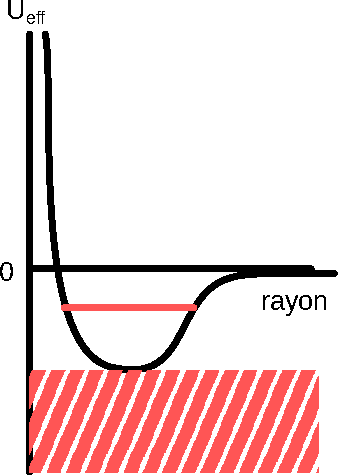
\includegraphics[scale=0.5]{ueff}
\subsection{Énergie mécanique négative}
On a alors \(e<1\).

On a \(l_1 = \frac{L*^2}{\mu k (1+e)}\) et \(l_2 = \frac{L*^2}{\mu k (1-e)}\)
\subsection{Nul}
On a alors \(e=1\) et on obeserve une parabole
\subsection{Négatif}
Si \(\cos(\varphi-\varphi_0)<-\frac{1}{e}\), on a \(\rho <0\), ce qui est impossible. On a alors une zone interdite \(\varphi \in [\varphi_0+\pi -\varphi_{min}, \varphi_0+\pi + \varphi_{min}]\) avec \(\varphi_{min} = \arccos(\frac{1}{e})\).
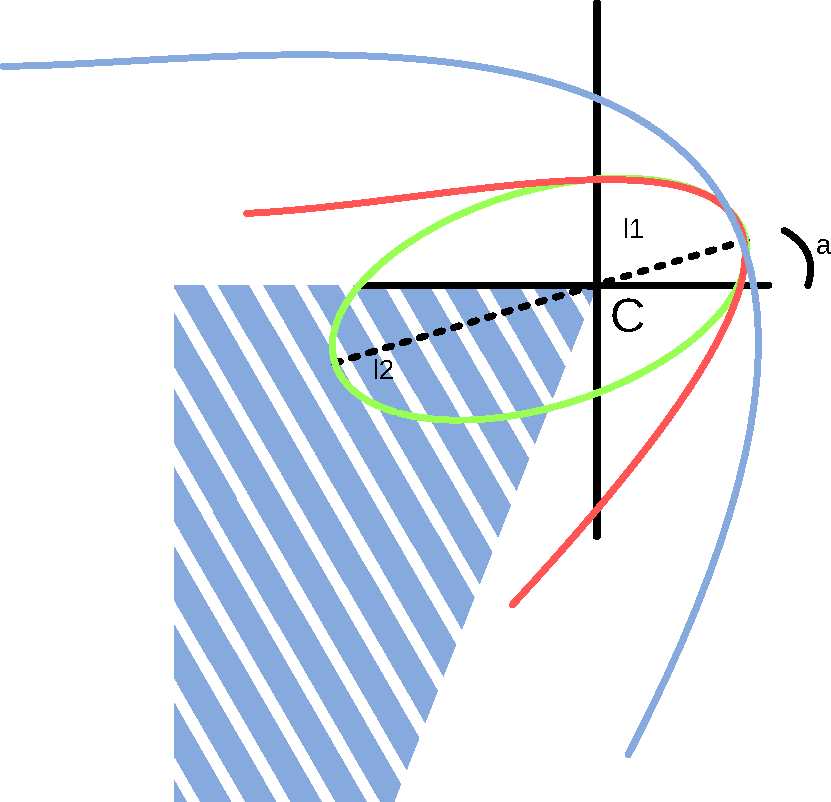
\includegraphics[scale=0.5]{mouv}
 \end{document}
